% !TeX program = pdflatex
\documentclass[border=6pt]{standalone}
\usepackage{tikz}
\usetikzlibrary{arrows.meta, positioning, calc}

\definecolor{MediumRed}{rgb}{0.925, 0.345, 0.345}
\definecolor{MediumGreen}{rgb}{0.37, 0.7, 0.66}
\definecolor{MediumBlue}{rgb}{0.015, 0.315, 0.45}
\definecolor{DarkBlue}{rgb}{0.05, 0.15, 0.35}

\def\s{0.30}

\begin{document}
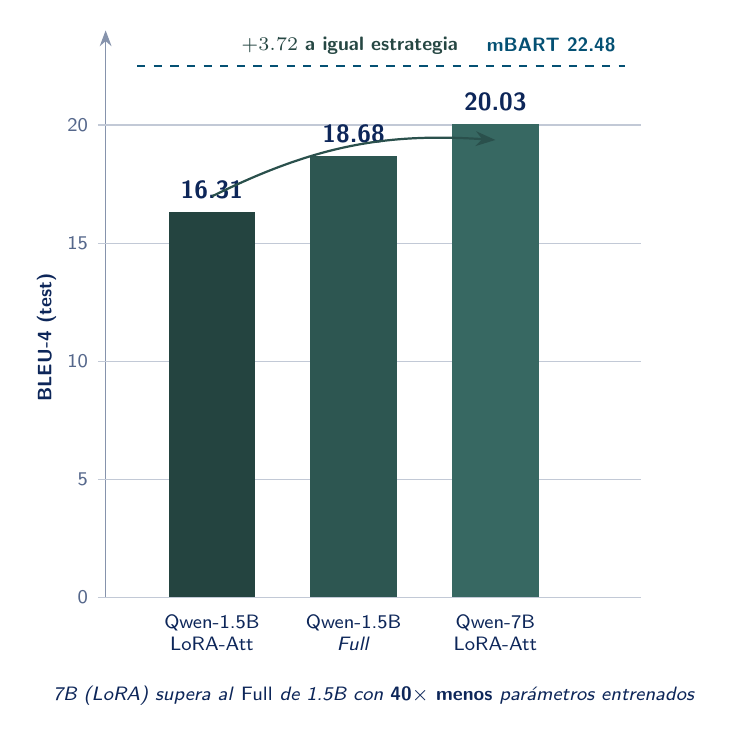
\begin{tikzpicture}[font=\sffamily]

% eje
\draw[DarkBlue!50, -{Stealth[length=2mm]}] (-0.4,0) -- (-0.4,{24*\s});
\foreach \y in {0,5,10,15,20}{
    \draw[DarkBlue!25] (-0.5,{\y*\s}) -- (6.4,{\y*\s});
    \node[font=\sffamily\scriptsize, text=DarkBlue!70, anchor=east] at (-0.5,{\y*\s}) {\y};
}
\node[font=\sffamily\scriptsize\bfseries, text=DarkBlue, rotate=90] at (-1.15,{11*\s}) {BLEU-4 (test)};

% barras
\foreach \x/\v/\c/\la/\lb in {%
    0.4/16.31/MediumGreen!38!black/{Qwen-1.5B}/{LoRA-Att},
    2.2/18.68/MediumGreen!48!black/{Qwen-1.5B}/{\emph{Full}},
    4.0/20.03/MediumGreen!58!black/{Qwen-7B}/{LoRA-Att}}{%
    \fill[\c] (\x,0) rectangle (\x+1.1,{\v*\s});
    \node[font=\sffamily\small\bfseries, text=DarkBlue, anchor=south] at (\x+0.55,{\v*\s+0.05}) {\v};
    \node[font=\sffamily\scriptsize, text=DarkBlue, anchor=north, align=center] at (\x+0.55,-0.1)
        {\la\\\lb};
}

% linea mBART
\draw[MediumBlue, dashed, thick] (0,{22.48*\s}) -- (6.2,{22.48*\s});
\node[font=\sffamily\scriptsize\bfseries, text=MediumBlue, anchor=east] at (6.2,{22.48*\s+0.28})
    {mBART 22.48};

% anotaciones
\draw[-{Stealth[length=2.5mm]}, MediumGreen!45!black, thick]
    (0.95,{16.31*\s+0.2}) to[bend left=15] (4.55,{20.03*\s-0.2});
\node[font=\sffamily\scriptsize\bfseries, text=MediumGreen!40!black, align=center] at (2.7,{20.03*\s+1.0})
    {$+3.72$ a igual estrategia};

\node[font=\sffamily\scriptsize\itshape, text=DarkBlue, align=center, anchor=north] at (3.0,-1.0)
    {7B (LoRA) supera al \emph{Full} de 1.5B con \textbf{40$\times$ menos} parámetros entrenados};

\end{tikzpicture}
\end{document}
